% Metódy inžinierskej práce

\documentclass[10pt,twoside,english,a4paper]{coursepaper}

\usepackage[english]{babel}
%\usepackage[T1]{fontenc}
\usepackage[IL2]{fontenc} % lepšia sadzba písmena Ľ než v T1
\usepackage[utf8]{inputenc}
\usepackage{graphicx}
\usepackage{url} % príkaz \url na formátovanie URL
\usepackage{hyperref} % odkazy v texte budú aktívne (pri niektorých triedach dokumentov spôsobuje posun textu)
\usepackage{copyrightbox}
\usepackage{caption}

\usepackage{cite}
\graphicspath{ {./images/} }
%\usepackage{times}
\newcommand{\source}[1]{\caption*{Source: {#1}} }

\pagestyle{headings}

\title{Loot boxes in video games and their link to problem gaming\thanks{Semestrálny projekt v predmete Metódy inžinierskej práce, ak. rok 2022/23, vedenie: MSc. Mirwais Ahmadzai}} % meno a priezvisko vyučujúceho na cvičeniach

\author{Jakub Bordáš\\[2pt]
	{\small Slovenská technická univerzita v Bratislave}\\
	{\small Fakulta informatiky a informačných technológií}\\
	{\small \texttt{xbordas@stuba.sk}}
	}

\date{\small 30. september 2022} % upravte



\begin{document}

\maketitle

\begin{abstract}
Loot boxes are crates in video games that contain randomised game content. Generally, adolescents are more prone to play video games. More than 2 billion people worldwide play video games for relaxation. To create more profit from their products, video game developers are implementing these loot boxes in their games. Every game in the TOP 5 leaderboard on SteamCharts.com (up to 04.10.2022) contains loot boxes. Creating more games with loot boxes creates an issue linking loot boxes with problem gambling. This article will focus more on the psychological features of loot boxes and how they should be regulated for young audiences or even deemed illegal.
\end{abstract}



\section{Introduction}

Motivujte čitateľa a vysvetlite, o čom píšete. Úvod sa väčšinou nedelí na časti.

Uveďte explicitne štruktúru článku. Tu je nejaký príklad.
Základný problém, ktorý bol naznačený v úvode, je podrobnejšie vysvetlený v časti~\ref{nejaka}.
Dôležité súvislosti sú uvedené v častiach~\ref{dolezita} a~\ref{dolezitejsia}.
Záverečné poznámky prináša časť~\ref{zaver}.



\section{What are lootboxes?} \label{what}

\begin{figure*}[tbh]
	\centering
	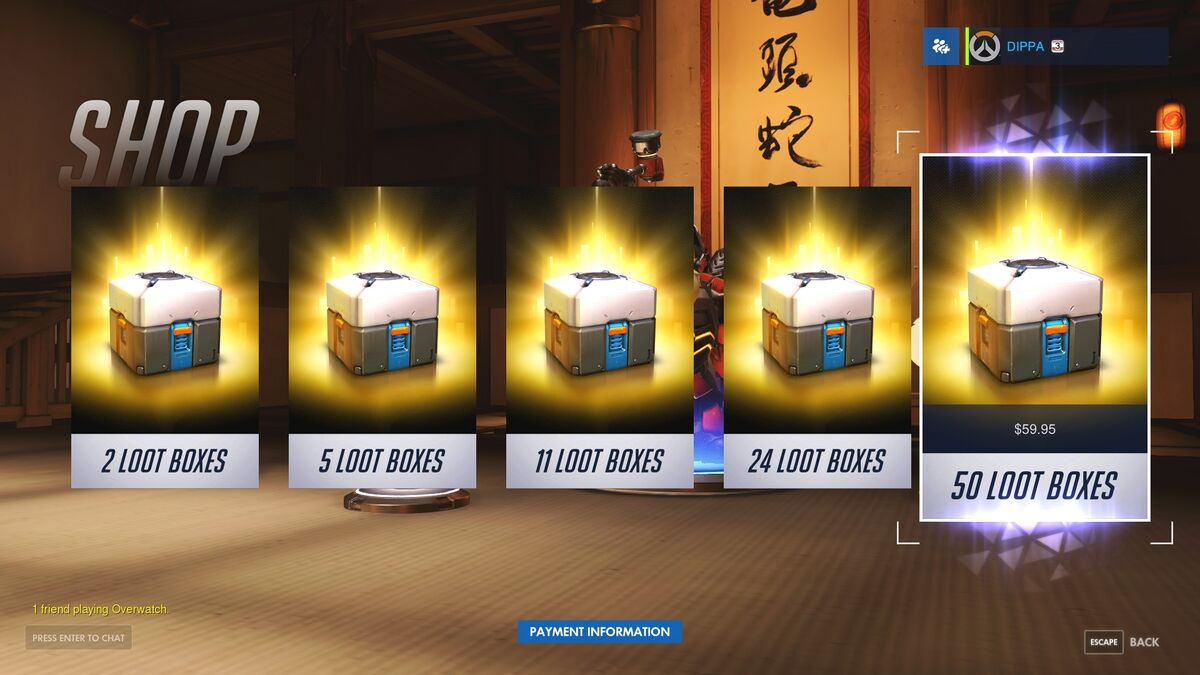
\includegraphics[scale=0.5]{img1}
	\caption{Loot boxes in Overwatch 1}
	\source{\url{https://crappygames.miraheze.org/wiki/Loot_box} }
	\label{fig:img1}
\end{figure*}

	Loot boxes are virtual containers in video games that contain one or more random rewards that alter the game in some way. Some can change your avatar aesthetic, unlock new levels or improve your in-game performance (e.g. via more powerful weapons or sets of armour). Possessing a unique avatar or powerful weapons is highly desirable. \par
	They are available for players to buy in popular games like Rocket League, Counter-Strike: Global Offensive, and League of Legends. Even more and more games tend to sell these loot boxes for real-world currency. In 2018 alone they generated approximately \$30 billion\cite{juniper:revenue}. This strategy has become a leading business model for generating profit from video games. \par
	The spread of loot boxes has raised the question of whether they should be regulated as a form of gambling. According to an article by Mark D. Griffiths, many of the loot box characteristics match those of gambling. The basic idea behind gambling is that an individual stakes money on the outcome of a future event, which is determined by chance in the hopes of receiving the desired reward. This would not be a problem if most players were not young teenagers and adolescents. 
	According to research\cite{springer:research} done on almost three thousand students in grades 7 to 12 in Ontario, most students (85\%) reported playing video games in the past year and almost 19\% reported playing video games daily. According to more recent source\cite{theesa:facts}, a total of 66\% of Americans play video games regularly. 
	




\section{Iná časť} \label{ina}

%Základným problémom je teda\ldots{} Najprv sa pozrieme na nejaké vysvetlenie (časť~\ref{ina:nejake}), a potom na ešte nejaké (časť~\ref{ina:nejake}).\footnote{Niekedy môžete potrebovať aj poznámku pod čiarou.}

%Môže sa zdať, že problém vlastne nejestvuje\cite{Coplien:MPD}, ale bolo dokázané, že to tak nie je~\cite{Czarnecki:Staged, Czarnecki:Progress}. Napriek tomu, aj dnes na webe narazíme na všelijaké pochybné názory\cite{PLP-Framework}. Dôležité veci možno \emph{zdôrazniť kurzívou}.


\subsection{Nejaké vysvetlenie} \label{ina:nejake}

Niekedy treba uviesť zoznam:

\begin{itemize}
\item jedna vec
\item druhá vec
	\begin{itemize}
	\item x
	\item y
	\end{itemize}
\end{itemize}

Ten istý zoznam, len číslovaný:

\begin{enumerate}
\item jedna vec
\item druhá vec
	\begin{enumerate}
	\item x
	\item y
	\end{enumerate}
\end{enumerate}


\subsection{Ešte nejaké vysvetlenie} \label{ina:este}

\paragraph{Veľmi dôležitá poznámka.}
Niekedy je potrebné nadpisom označiť odsek. Text pokračuje hneď za nadpisom.



\section{Dôležitá časť} \label{dolezita}




\section{Ešte dôležitejšia časť} \label{dolezitejsia}




\section{Záver} \label{zaver} % prípadne iný variant názvu



%\acknowledgement{Ak niekomu chcete poďakovať\ldots}


% týmto sa generuje zoznam literatúry z obsahu súboru literatura.bib podľa toho, na čo sa v článku odkazujete
\bibliography{literatura}
\bibliographystyle{abbrv} % prípadne alpha, abbrv alebo hociktorý iný
\end{document}
